\section{Sorting problem}

The sorting problem is a fundamental computational task in which a collection of elements is arranged in a specific order, typically ascending or descending. 
Given an unsorted list or array, the goal is to rearrange the elements to follow a predefined sequence based on a chosen criterion, such as numerical or lexicographical order. 

\subsection{Quicksort}
Quicksort, introduced by Hoare in 1962, is a highly efficient, in-place, divide-and-conquer sorting algorithm known for its practical performance across a variety of applications.
By partitioning data around a pivot element, Quicksort can achieve efficient sorting with minimal extra storage, making it one of the most widely used sorting algorithms.

The Quicksort algorithm works as follows:
\begin{enumerate}
    \item \textit{Divide}: select a pivot element from the array, then partition the array into two subarrays. 
        Elements less than or equal to the pivot form the left subarray.
        Elements greater than or equal to the pivot form the right subarray.
    \item \textit{Conquer}: recursively apply Quicksort to each of the two subarrays.
    \item \textit{Combine}: since the subarrays are sorted in place, no additional merging is needed.
\end{enumerate}
The efficiency of Quicksort depends on the partitioning step, which operates in $\mathcal{O}(n)$ time. 
\begin{algorithm}[H]
    \caption{Quicksort}
    \begin{algorithmic}[1]
        \Function{partition}{$A,p,q$}
            \State $x=A[p]$
            \State $i=p$
            \For {$j=p+1$\textbf{ to }$q$}
                \If {$A[j]\leq x$}
                    \State {$i=i+1$}
                    \State \textbf{exchange }$A[i]$ and $A[j]$
                \EndIf
            \EndFor
            \State \textbf{exchange }$A[p]$ and $A[i]$
            \State \Return $i$
        \EndFunction
        \Statex
        \Procedure{Quicksort}{$A,p,r$}
            \If {$p<r$}
                \State $q=$ \Call{partition}{$A,p,r$}
                \State \Call{Quicksort}{$A,p,q-1$}
                \State \Call{Quicksort}{$A,q+1,r$}
            \EndIf
        \EndProcedure
    \end{algorithmic}
\end{algorithm}  
The performance of Quicksort varies based on the choice of pivot and the input data. 
Here are the primary cases:
\begin{itemize}
    \item \textit{Worst-case}: the pivot always ends up at one of the ends of the array, resulting in highly unbalanced partitions.
        This scenario, often due to already sorted or reverse-sorted data when a poor pivot is chosen, yields a time complexity of $\Theta(n^2)$.
    \item \textit{Average case}:  the pivot splits the array into reasonably balanced parts.
        This is achieved with a random or median pivot selection, leading to a time complexity of $\Theta(n \log n)$, which is efficient for large datasets.
    \item \textit{Best case}: the pivot consistently splits the array into two equal halves, minimizing the depth of recursive calls. 
        This optimal scenario also results in a time complexity of $\Theta(n \log n)$.
\end{itemize}

\subsection{Randomized Quicksort}
Randomized Quicksort is an improved variant of the classic Quicksort algorithm that selects a pivot randomly from the array, significantly reducing the chance of worst-case performance.
By ensuring the pivot choice is independent of the input structure, Randomized Quicksort achieves efficient performance on average for various inputs.

The randomized selection of the pivot minimizes the probability of consistently poor partitions, where the pivot might otherwise split the array in highly unbalanced ways. 
With a randomized pivot, the expected time complexity becomes $\Theta(n \log n)$, independent of any initial ordering of the data.

\paragraph*{Analysis}
Let $X$ denote the running time of Randomized Quicksort on an input of size $n$, assuming that each pivot selection is independent and uniformly random. 
Define an indicator variable $X_k$ for the event that a partition results in a split of $k$ elements on one side and $n-k-1$ elements on the other:
\[X_k=\begin{cases}
    1 \qquad \text{if PARTITION generates a } k \mid (n-k-1) \text{ split} \\
    0 \qquad \text{otherwise}
\end{cases}\]
Since any element can be chosen as the pivot with equal probability, the expected value of $X_k$ is: 
\[\mathbb{E}[X_k] = \Pr(X_k = 1) = \dfrac{1}{n}\]
Thus, the expected running time $\mathbb{E}[T(n)]$ can be written in terms of the recursive costs of partitioning:
\[\mathbb{E}[T(n)] = \mathbb{E} \left[ \sum_{k=0}^{n-1} X_k \left( T(k) + T(n - k - 1) + \Theta(n) \right) \right]\]
This simplifies to:
\[\mathbb{E}[T(n)] =\frac{2}{n} \sum_{k=1}^{n} \mathbb{E}[T(k)] + \Theta(n)\]

For sufficiently large $n \geq 2$, this recursive relation leads to:
\[\mathbb{E}[X]\leq \frac{2}{n} \sum_{k=1}^{n} ak\log k + \Theta(n)\leq an\log n\]
Thus, for a sufficiently large constant $a$, the $\Theta(n)$ term is dominated, leading to an overall time complexity of:
\[\mathcal{O}(n\log n)\]

\paragraph*{Practical performance}
In practice, Randomized Quicksort often outperforms Merge Sort, typically running at least twice as fast due to its efficient in-place operations and reduced memory usage. 
With careful code tuning and optimized implementations, Quicksort's performance can be further enhanced. 
Its contiguous memory access patterns make it highly cache-friendly, and it handles virtual memory effectively.

\subsection{Comparison sort analysis}
All the sorting algorithms discussed so far are comparison sorts, where element ordering is determined by comparing pairs of elements. 
The best worst-case time complexity for these algorithms is $\mathcal{O}(n\log n)$. 

To understand this lower bound, consider sorting an array $\left\langle a_1,a_2,\dots,a_n\right\rangle$. 
We can represent each sequence of comparisons made by a sorting algorithm as a path in a decision tree:
\begin{itemize}
    \item Each internal node in this tree represents a comparison between two elements $a_i$ and $a_j$.
    \item The left child of a node represents the branch taken if $a_i \leq a_j$, while the right child represents the branch if $a_i > a_j$. 
\end{itemize}
Each leaf node in the decision tree corresponds to a unique, final sorted order (or permutation) of the array. 
Therefore, this tree models all possible sequences of comparisons that could occur for different input configurations.
\begin{example}
    Consider sorting the array $\left\langle 9,4,6\right\rangle$. 
    A decision tree for this array might look as follows, showing different comparison paths:
    \begin{figure}[H]
        \centering
        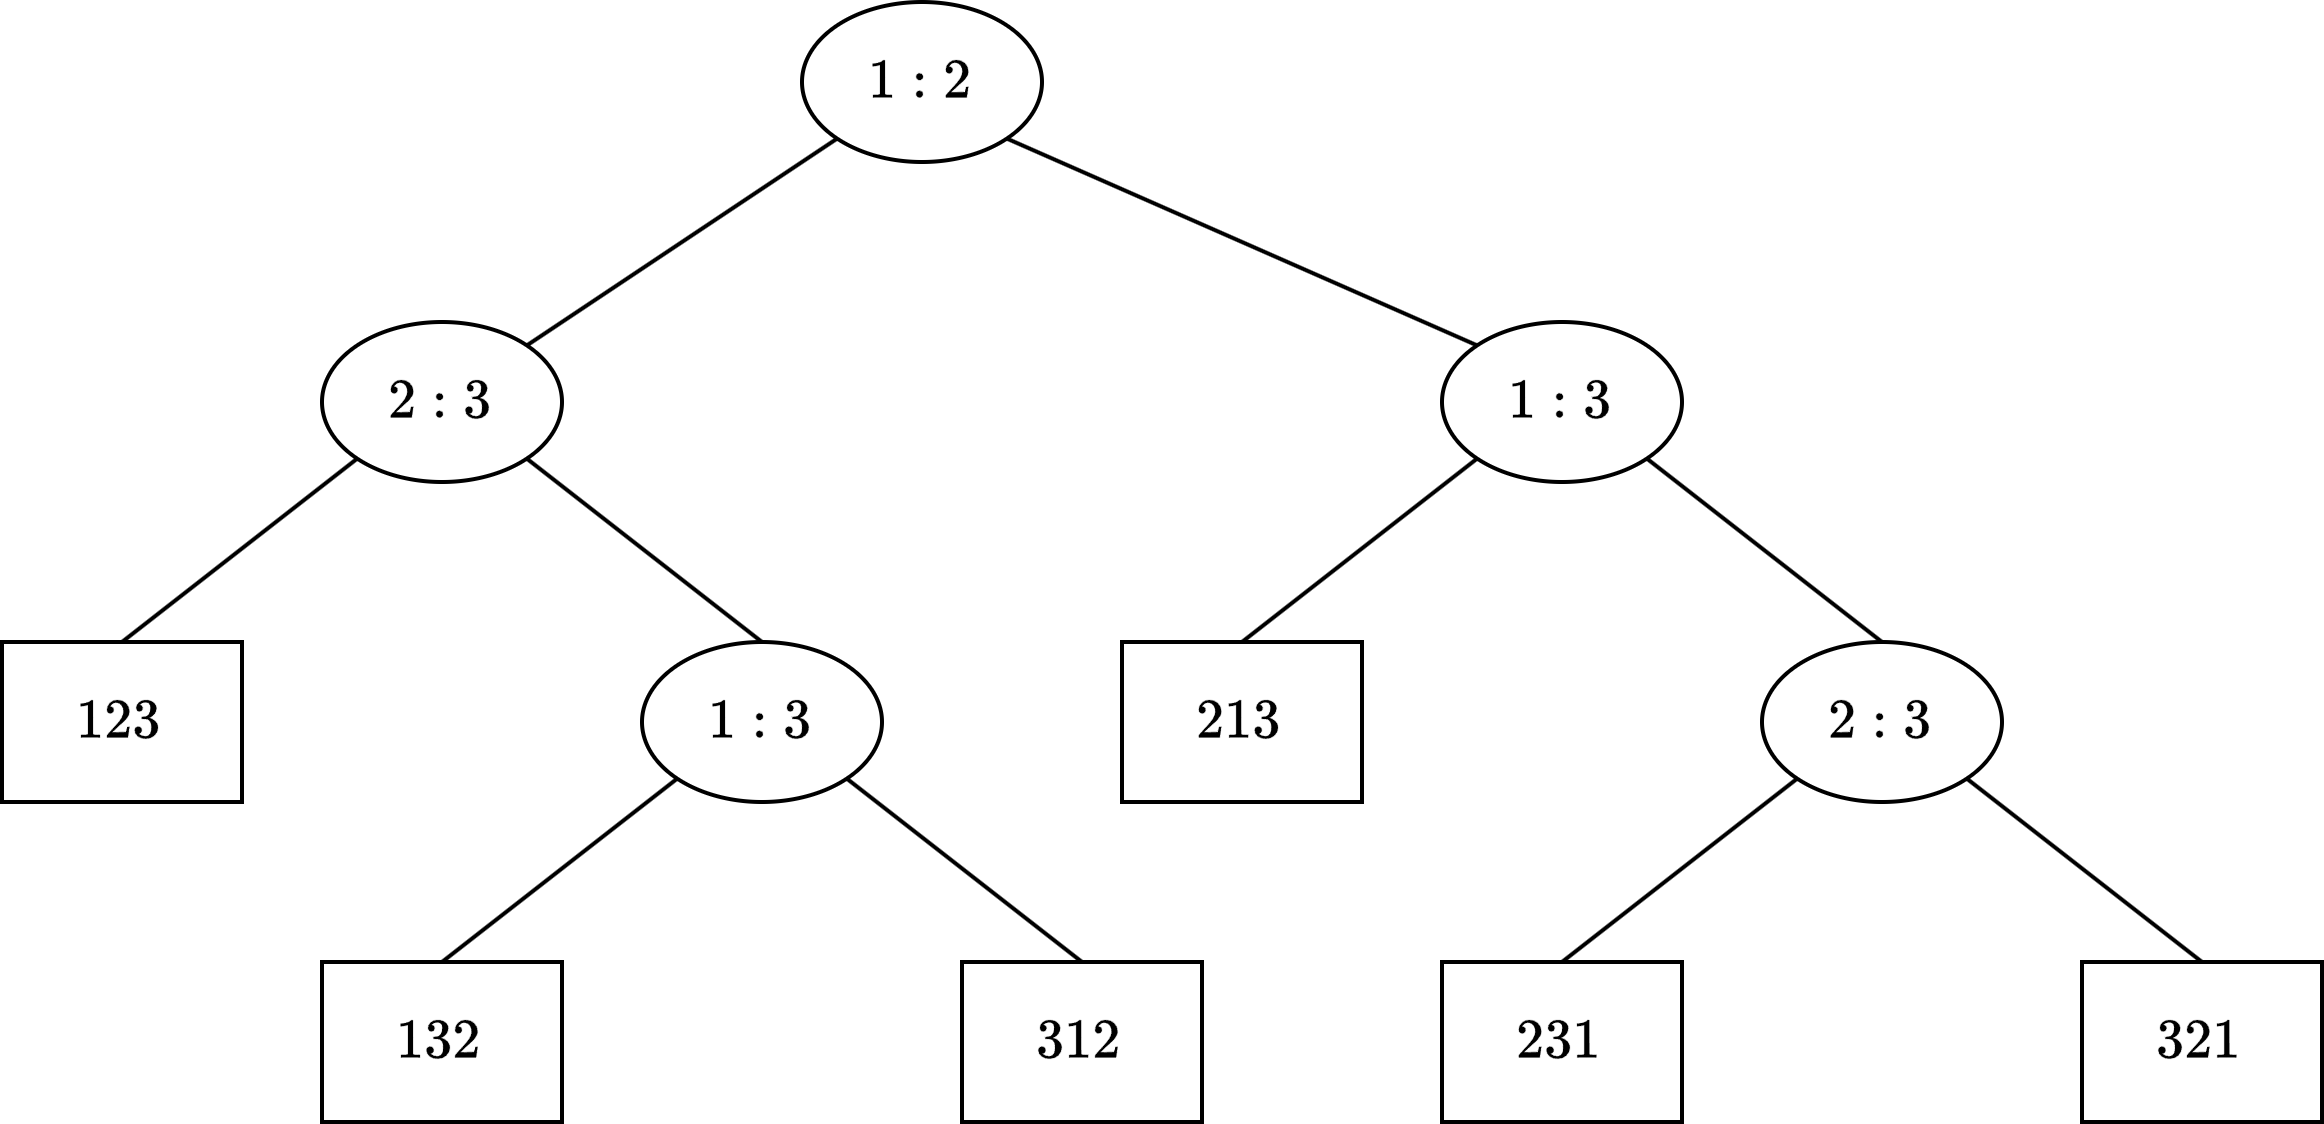
\includegraphics[width=0.8\linewidth]{images/tree1.png}
    \end{figure}
\end{example}
The height of the decision tree represents the worst-case number of comparisons needed to sort the array, which corresponds to the algorithm's worst-case running time.
Since there are $n!$ possible ways to order $n$ distinct elements, the decision tree must have at least $n!$ leaves to account for every possible permutation.

For a binary tree of height $h$, the maximum number of leaves is $2^h$, so we must have:
\[2^h\geq n!\]
Taking the logarithm of both sides and applying Stirling's approximation, $n!\approx\left(\frac{n}{e}\right)^n$, we get:
\[\log n!\geq n\log n-n\log e\]
Thus, the minimum height $H(n)$ of the decision tree is:
\[H(n)=\Omega(n\log n)\]
This proves that any comparison-based sorting algorithm has a worst-case time complexity of $\Omega(n\log n)$.
\begin{theorem}
    Any decision tree that can sort $n$ elements must have height $\Omega(n \log n)$.
\end{theorem}
\begin{corollary}
    Heapsort and Merge Sort achieve this asymptotic lower bound, making them optimal comparison-based sorting algorithms.
\end{corollary}

\subsection{Counting sort}
Counting sort is a non-comparison-based sorting algorithm that efficiently organizes elements by leveraging their value range rather than making direct comparisons between them.
This makes it particularly useful for sorting arrays with integer elements drawn from a small range of possible values.

\paragraph*{Algorithm}
Counting sort takes as input an array $A[n]$, where each element $A[j]\in\{1, \dots, k\}$, and returns a sorted array $B[n]$.
The algorithm also requires an auxiliary array $C[k]$ for counting the frequency of each element in $A[n]$. 

The Counting Sort algorithm works in the following steps:
\begin{enumerate}
    \item \textit{Initialize the counting array}: initialize an array $C$ of size $k$, where each element is initially set to zero. 
        This array will store the frequency of each element in $A$.
    \item \textit{Count the occurrences}: traverse the input array $A$, and for each element A[j], increment the corresponding position in array $C$.
    \item \textit{Compute the prefix sum}: update array $C$ by converting it to a prefix sum array. 
        This allows the algorithm to determine the final position of each element in the sorted output.
    \item \textit{Build the sorted array}: iterate through the input array $A$ in reverse order, and place each element at its correct position in the output array $B$, using the values in $C$ for positioning. 
        As elements are placed into $B$, decrement their corresponding counts in $C$.
\end{enumerate}
\begin{algorithm}[H]
    \caption{Counting Sort}
    \begin{algorithmic}[1]
        \For{$i=1$ \textbf{ to } $k$} \Comment Set all elements of array $C$ to zero.
            \State $C[i]=0$ 
        \EndFor \Comment Complexity $\Theta(k)$
        \For{$j=1$ \textbf{ to } $n$} \Comment Count how many times each element appears in the input array $A$
            \State $C[A[j]]=C[A[j]]+1$ 
        \EndFor \Comment Complexity $\Theta(n)$
        \For{$i=2$ \textbf{ to } $k$} \Comment Compute the prefix sum for each element in $C$
            \State $C[i]=C[i]+C[i-1]$ 
        \EndFor \Comment Complexity $\Theta(k)$
        \For{$j=n$ \textbf{ to } $1$} \Comment Place elements into output array $B$ and reduce counters in $C$
            \State $B[C[A[j]]]=A[j]$
            \State $C[A[j]]=C[A[j]]-1$ 
        \EndFor \Comment Complexity $\Theta(n)$
    \end{algorithmic}
\end{algorithm}  
\begin{example}
    Let's consider an example where we sort the array $A=\left\langle 4, 1, 3, 4, 3\right\rangle$, with $k=4$. 
    \begin{enumerate}
        \item \textit{Initial state}: initialize the array $C$ to all zeros: $C=\left\langle 0,0,0,0\right\rangle$.
        \item \textit{Count elements}: count the occurrences of each element in $A$, resulting in: $C=\left\langle 1,0,2,2\right\rangle$.
        \item \textit{Compute the prefix sum}: compute the prefix sum over $C$: $C=\left\langle 1,1,3,5\right\rangle$.
        \item \textit{Place elements into output array}: starting from the last element of $A$, place elements into their correct position in $B$ using the cumulative counts in $C$, and decrement the counts as we go. 
            The final result will be: $B=\left\langle 1,3,3,4,4\right\rangle$ and $C=\left\langle 0,1,1,3\right\rangle$.
    \end{enumerate}
\end{example}
The time complexity of Counting Sort is the sum of the complexities of each of the four loops
\[\mathcal{O}(n)+\mathcal{O}(k)+\mathcal{O}(n)+\mathcal{O}(k)=\mathcal{O}(n+k)\]
If $k = \mathcal{O}(n)$, then counting sort runs in linear time: 
\[\Theta(n)\]
\begin{definition}[\textit{Stable sorting algorithm}]
    A sorting algorithm is called stable if it preserves the relative order of equal elements from the input array.
\end{definition}
\begin{property}
    Counting Sort is a stable sort.
\end{property}





























\subsection{Radix sort}
Radix sort is a non-comparative sorting algorithm that sorts numbers digit by digit, starting from the least significant digit to the most significant digit. 
It can be highly efficient for large datasets when certain conditions are met.

The idea behind radix sort is to process each digit of the numbers, from the least significant to the most significant, sorting them progressively by each digit's place value. 
This approach avoids direct comparisons between elements, making it suitable for sorting large datasets when combined with a stable auxiliary sorting algorithm.

Assume the numbers have already been sorted by the least significant $t-1$ digits.
Now, sort the numbers based on the $t$-th digit. 
If two numbers differ in the $t$-th digit, they will be correctly ordered after the pass.
If they are identical in the $t$-th , they retain their relative order due to the stability of the auxiliary sort.

\paragraph*{Algorithms}
The teps for radix sort are: 
\begin{itemize}
    \item \textit{Sort by least significant digit}: sort the numbers based on the least significant digit, using a stable sorting algorithm like counting sort.
    \item \textit{Iterate through remaining digits}: repeat the sorting process for each more significant digit, ensuring that the relative order of numbers is maintained between passes.
    \item \textit{Final order}: after all digits have been processed, the numbers are fully sorted.
\end{itemize}

\paragraph*{Analysis}
To analyze the efficiency of radix sort, we assume that counting sort is used as the stable sorting method for each digit. 
Suppose we are sorting $n$ integers, where each integer is represented by $b$ bits. 
Each integer can be thought of as having $\frac{b}{r}$ digits, where each digit is based on $2^r$ possible values.
Each pass of counting sort processes $n$ elements and sorts them based on a single digit, requiring $\Theta(n + 2^r)$ time. 
Since there are $\frac{b}{r}$ passes (each pass sorting based on one digit), the overall time complexity of radix sort is:
\[T(n)=\Theta\left(\dfrac{b}{r}(n+2^r)\right)\]

\paragraph*{Optimization}
To optimize radix sort, we aim to minimize the total running time. 
Increasing $r$, the number of bits used for each digit, reduces the number of passes $\frac{b}{r}$, but it also increases the cost of processing each digit, as $2^r$ grows exponentially.

For optimal efficiency, we want to avoid letting $2^r$ exceed $n$, since this would lead to unnecessary overhead.
For efficiency, we should avoid letting $2^r>n$.

The optimal choice for $r$ is typically $r=\log n$, as it balances the number of passes and the digit processing cost.
Thus, the overall time complexity becomes:
\[T(n,b)=\Theta\left(\dfrac{bn}{\log n}\right)\]

\paragraph*{Considerations}
In practice, radix sort is particularly efficient for large datasets, especially when the number of digits is relatively small compared to the number of elements. 
It is simple to implement and does not require comparisons between elements. 
However, radix sort has poorer cache locality and memory access patterns compared to algorithms like Quicksort, which can negatively affect performance for smaller datasets or systems with limited memory bandwidth.